\chapter{Must-Alias Analysis: Data Structures}
\label{chapter:must-data}
\epigraph{I love humans. Always seeing patterns in things that aren’t there.}{\textit{The 8th Doctor} - Doctor Who}

The previous chapter presented an elegant minimal model of a must-alias analysis in the declarative setting of Datalog (and the \doop{} framework). Although attractive in its expressiveness, if the model is to be implemented as is it will incur serious performance penalties. As mentioned in the discussion Section~\ref{sec:must-logic:equivalence}, an important prerequisite for a must-alias analysis is that of encoding equivalence classes on access paths. Datalog inherently offers no feature to support such notion and thus, in the previous chapter, we had to resort to an explicit representation of all alias pairs.

In this chapter, we present a data structure that can dramatically speed up the performance of must-alias analysis. The insights behind the data structure are quite general. First, the fact that must-alias sets are equivalence classes and the need to avoid explicitly computing each alias pair. In contrast, an optimized implementation will encode aliasing implicitly: as membership in the same sub-structure. This is a technique also employed in past static analysis approaches in different settings (e.g., in the use of union-find trees in Steensgaard-style~\cite{popl:1996:Steensgaard} points-to analysis). Additionally, aliasing can be implicitly extended to longer access paths and this inference should be readily computable in the course of the analysis. For instance, if two program expressions \code{x} and \code{y.next} are aliases, then so are all their extensions (e.g., \code{x.prev} and \code{y.next.prev}). Such ``derivative'' relationships should be represented compactly. In our data structure, we represent complex program expressions implicitly until expansion is needed and up to the extent that must-alias information exists for them.

Our data structure is effectively a symbolic abstraction of the program's heap---as a directed graph. We invent for each variable a graph node: an abstract object that represents ``the object that the variable points to''. Although several abstractions of the heap have appeared in the literature, ours is distinguished by several elements---e.g., a mere ``load'' operation introduces a new abstract object. An abstract object in our structure represents at most one concrete object, unlike traditional abstractions that map multiple concrete objects to one abstract. Whenever a must-alias inference is made, the corresponding abstract objects are merged: the two abstract objects have to correspond to the same concrete one. Access paths are represented implicitly, as regular paths that follow object fields through our symbolic heap. All operations over the graph arising during a must-alias analysis (especially the intersection of graphs) are performed highly efficiently.

We implement the data structure in two settings: imperatively, in Java, with destructive updates (upon aliasing, abstract objects are collapsed together) and purely functionally (upon aliasing, abstract objects are related in an associative structure). The latter is suitable for a declarative implementation, in the Datalog language. We show that the data structure yields large performance improvements compared to an explicit representation of alias pairs. The imperative version achieves a speedup of up to two orders of magnitude, with the declarative implementation nearly matching it in most cases. As a result, the running time of a realistic must-alias analysis becomes small---a few tens of seconds for large benchmarks and the full Java library.

Overall, in this chapter we:

\begin{itemize}
\item Describe the primitive operations (e.g., set intersection) that a must-alias analysis needs to perform.
\item Present an efficient data structure for representing must-alias analysis inferences and efficiently encode operations over that structure.
\item Apply the new data structure on an must-alias analysis implemented in an existing framework and quantify the benefits in different implementation settings.
\end{itemize}


\section{Must-Alias Analysis Needs}
\label{sec:must-data:needs}

Before presenting our optimized data structure for a must-alias analysis, it is important to ponder upon the properties of such an analysis and the algorithmic needs that arise if one is to implement it with performance in mind. The previous section offered a minimal yet representative Datalog model of a must-alias analysis. A great benefit of a distilled declarative model is the ability to reason about its properties. Directly executing the Datalog rules of Section~\ref{sec:must-logic:model} is a realistic proposition. Indeed, the must-alias analysis in the \doop{} framework is well-captured by the model. However, several inefficiencies arise from the rules. We next examine the model and discuss how it leads to an optimized data structure, and its associated algorithms, for must-alias analysis.


\paragraphhead{Representing Equivalence Relations.}
We have already commented on the effects of a naive implementation of the must-alias relation in previous sections. For instance, four program expressions aliasing with each other would require the explicit representation of twelve alias pairs (ignoring the trivial pairs of each expression aliasing with itself) in order for the relation to stay reflexive, symmetric and transitively closed.

Since must-alias is an equivalence relation, it induces a partitioning of the space of access paths: every access path can only belong in one alias (equivalence) class. This means that we can represent the contents of each class compactly, by grouping together all aliased access paths. An access path can denote that it belongs in a certain alias class, e.g., by having a unique identifier, or by being a member in a linked data structure. The goal is to represent an alias class using linear space and time (in the number of its access paths) instead of enumerating all pairs of aliased access paths (and taking up quadratic space and time).

It is important to note that the concrete (i.e., dynamic) ``alias'' relation is also an equivalence relation, but most \emph{may}-alias relations in the static analysis literature are \emph{not}. For instance, in a typical subset-based pointer analysis, access path \code{ap1} may-alias \code{ap2} by pointing to the same abstract object (among others). Similarly, \code{ap2} may-alias \code{ap3}. However, it may not be the case that \code{ap1} and \code{ap3} may-alias: the common elements in the points-to sets of \code{ap1} and \code{ap2} may not be among the common elements in the points-to sets of \code{ap2} and \code{ap3}. This highly influences all data structure operations. Notably, the main algorithm that we will describe (intersection of data structures when joining control-flow paths) is not present in a may analysis.


\paragraphhead{Extending Access Paths.}
A less obvious observation concerns the representation of aliasing in extended access paths. A naive implementation would, once again, have to represent aliases explicitly. For instance, two aliased program variables \code{x} and \code{y} will also induce alias pairs \code{x.f} and \code{y.f}, as well as \code{x.g} and \code{y.g}, \code{x.f.g} and \code{y.f.g}, etc., up to the maximum access path length (and modulo valid field accesses). This is an exponential number, $\Omega(c^k)$, of aliased access paths, for $c$ valid fields and access path length limit of $k$. The access path length can be easily limited (e.g., $k = 3$ does not restrict the vast majority of useful alias inferences), so the burden is not insurmountable, but it can still be significant.

Ideally, we would like a data structure that only explicitly maintains the initial aliasing relationship and can implicitly derive the aliasing of all extended access paths.


\paragraphhead{Algorithms.}
Once we have a data structure that satisfies the above requirements, what algorithms should we implement efficiently on this data structure? The basic algorithms behind most must-alias analysis inferences are straightforward. The analysis needs to copy alias classes (equivalence classes), add a single access path, remove a single access path, or rename variables in a set of alias classes. The only case that introduces some complexity is the one dealing with multiple predecessors of an instruction in the control-flow graph.

In a must-alias analysis setting, in order for an alias pair to be valid at the instruction where multiple control-flow paths meet, it should hold in each path. The operation we need here is that of taking the intersection of alias classes from many different sets (one for each predecessor instruction). For instance, in the code snippet of Figure~\ref{fig:must-data:snippet}, on line 19, we can infer that \{\code{a2.member} $\sim$ \code{b1}\} since it holds in both paths, but not that \{\code{a2.next} $\sim$ \code{a1}\}.

\begin{figure}[htb!p]
\begin{subfigure}{.45\textwidth}
\begin{javacode}
class A { 
    A next;
    B member;
    A(A next, B member) {
        this.next = next;
        this.member = member; } }
class B {
    A container;
    B(A container) {
        this.container = container; } }
\end{javacode}
\end{subfigure}%
\hfill
\begin{subfigure}{.45\textwidth}
\begin{javacode*}{firstnumber=11}
void main(String[] args) {
    B b1 = new B(null);
    A a1 = new A(null, b1);
    A a2;
    if (args != null) 
        a2 = new A(null, b1);
    else
        a2 = new A(a1, b1);
    b1.container = a2;
}
\end{javacode*}
\end{subfigure}
\caption[Code snippet for illustrating the data structure algorithms]{Code snippet to illustrate certain points of our algorithms.}
\label{fig:must-data:snippet}
\end{figure}


\paragraphhead{More than a Union-Find.}
Before describing our data structure in full detail, it is important to note how it differs from an implementation of the well known \emph{Union-Find} data structure. First, it extends on the idea of keeping sets of equivalent elements, by connecting equivalence classes in order to form complex access paths in a compact way. Secondly, it allows for deletions of elements from an equivalence class, potentially producing sets without elements (but significantly different to an empty set---as explained later). Thirdly, and more importantly, our data structure introduces an additional operation on equivalence classes---that of \emph{intersection}---in supplement to that of \emph{union}.

Notably, in contrast to a typical data structure for equivalence classes, unions of (non-singleton) equivalence classes do not arise: if an expression is newly aliased with others, it is because it is no longer aliased with its previous aliases. The corresponding operation is a single access path addition and removal (from a different class). Conversely, intersections of alias classes are central to our structure.


\section{An Optimized Data Structure and Algorithms}

Based on the above requirements, we propose an \emph{alias graph} data structure (and associated algorithms) for representing all alias sets of access paths that hold at a certain program point. In a typical must-alias analysis, a program point is a possibly context-qualified instruction. Each such \emph{instruction-and-context} combination maintains an alias graph and the analysis updates it until fixpoint. An updated alias graph depends on the earlier graph for the same program point, on the graphs of its predecessor instructions, and on the current instruction's semantics.

We begin with a description of the easier case: how the current instruction affects the alias graph. This will also help illustrate the data structure.

The intuition is that an alias graph abstractly represents local variables and the heap, with abstract objects as placeholders for concrete objects. Nodes (abstract objects) are alias classes, edges are field-points-to relationships. Every abstract object, however, corresponds to (at most) a single concrete object at the current program point: our data structure is isomorphic with a part of the concrete heap. This property is true only because the data structure represents definite (must) aliasing.

We illustrate with simple examples. It is worth noting once again that every program instruction will maintain a different alias graph. The following examples focus on the situation at a certain instruction.

All variables conceptually begin with their own node in the graph. (In practice, such nodes need not be represented, unless connected to others.) The node represents ``the object that the variable points to at this program point''.

\begin{figure*}[ht]
\centering
% left bottom right top
\includegraphics[trim={35mm 115mm 35mm 51mm},clip,width=0.8\linewidth]{assets/must-data/alias-graph0.pdf}
\end{figure*}

Aliasing can be induced by various program operations (e.g., \relname{Move}, \relname{Load}, and \relname{Store}), as seen in our earlier model. Since we are interested in must-alias, two aliased variables have to point to the same object---their nodes can be merged if a \relname{Move} instruction, \code{x = y}, is encountered:

\begin{figure*}[ht]
\centering
% left bottom right top
\includegraphics[trim={35mm 115mm 35mm 51mm},clip,width=0.8\linewidth]{assets/must-data/alias-graph1.pdf}
\end{figure*}

This collapsing of nodes is responsible for compact encoding of equivalence relations: two variables are computed to be aliases iff\footnote{The statement refers to the must-alias analysis results, not to actual aliasing during program execution.} they belong in the same node of the alias graph.

If the next instruction is a \relname{Store}, \code{x.f = z}, the previous graph will get propagated---i.e., copied. Subsequently, the \relname{Store} will add an edge to the graph, signifying that the field, \code{f}, of the object pointed by \code{x} will point to the object that \code{z} points to:

\begin{figure*}[ht]
\centering
% left bottom right top
\includegraphics[trim={35mm 115mm 35mm 51mm},clip,width=0.8\linewidth]{assets/must-data/alias-graph2.pdf}
\end{figure*}

A subsequent \relname{Load} operation, \code{z = y.g},\footnote{The example sequence of actions described is contracted for brevity. Our implementation works on a static single assignment (SSA) intermediate form, so this exact scenario will never arise, since \code{z} has had its value read earlier and its single assignment has to dominate its use.} will inherit the alias graph of its predecessor and will modify it. Variable \code{z} is removed from its old node (\code{z} no longer points to this abstract object), a new node for \code{z} is created, and the nodes are linked, to indicate that \code{z} now points to the same object as \code{y.g}. The empty, former node of \code{z} will be garbage collected if no other paths can reach it in the alias graph.

On the other hand, when an access path can still reach the empty node, the empty node provides useful information. It represents ``the object that an access path points to at this program point''. Empty here doesn't describe the lack of information---just the lack of a \emph{local variable} pointing to this abstract object.

\begin{figure*}[ht]
\centering
% left bottom right top
\includegraphics[trim={35mm 85mm 35mm 51mm},clip,width=0.8\linewidth]{assets/must-data/alias-graph3.pdf}
\end{figure*}

The \relname{Load} operation shows that our alias graph, although intended to abstractly represent a real heap, behaves quite differently: a load from a field can introduce new objects, as well as update fields of existing objects.

Generally, the alias graph captures compactly all aliasing relationships among access paths. Maintaining the graph across program instructions is simple, as in the above examples. Graph manipulation merely has to observe some invariants:

\begin{itemize}
\item Two variables are in the same graph node iff the analysis reports them to be aliased. (Since alias classes are disjoint, the variables in different nodes are also disjoint.)

\item A path in the graph represents a set of access paths, starting from a non-empty node (that denotes the base variables of the access paths) and extended with the field labels along the path's edges. If two paths in the graph reach the same node, all access paths they represent must be aliased.
\end{itemize}

For illustration, consider Figure~\ref{fig:must-data:alias-graph}, which shows the alias graph after line 19 of our code example in Figure~\ref{fig:must-data:snippet}.

\begin{figure}[ht]
\centering
\includegraphics[trim={13mm 15mm 10mm 10mm},clip,width=0.7\linewidth]{assets/must-data/alias-graph.pdf}
\caption[Example alias graph data structure]{Example alias graph data structure.}
\label{fig:must-data:alias-graph}
\end{figure}

The graph concisely represents a set of alias relationships that hold at that program point: \{\code{b1.container} $\sim$ \code{a2}\}, \{\code{a1.member} $\sim$ \code{b1}\}, and \{\code{a2.member} $\sim$ \code{b1}\}. An infinite number of other alias pairs are represented implicitly: \{\code{a1.member} $\sim$ \code{a2.member}\}, \{\code{a1.member.container} $\sim$ \code{a2}\}, \{\code{a1.member.container.member} $\sim$ \code{b1}\}, \{\code{a1.member.container.member} $\sim$ \code{a1.member}\}, etc.

Overall, the alias graph satisfies both of our requirements of Section~\ref{sec:must-data:needs} for an efficient representation. Equivalence relations are represented compactly: an alias class with $n$ members does not need $O(n^2)$ space and time for its computation. Instead, it is represented implicitly, as all the variables in a node ($O(n)$ space) and all alias graph paths that can reach a node. Similarly, long (and even infinite) access paths are represented implicitly as graph paths. The implicit representation is sufficient for any specific queries (i.e., ``are two given program expressions aliases?'') and for subsequent aliasing computations, per the algorithms we detail next.


\subsection{Main Algorithms}

Most of the required must-alias analysis actions (per the discussion of Section~\ref{sec:must-data:needs}) over our data structure are straightforward, consisting of copying, additions and removals of variables and edges, and variable renamings. Standard mappings for efficient indexing are required: each target of a directed edge needs to be able to quickly retrieve its source, and each program variable needs to quickly map to the node in which it appears. 

For instance, according to the earlier definition of the data structure, finding all aliases of an access path is simple (but requires a transitive computation---our graph is a condensed representation of alias classes):


\paragraph{Algorithm: \rel{all-aliases}{ap}}
\begin{itemize}
\item Find the node for the base variable of access path \args{ap}, traverse in the forward direction the labeled edges that match each of the fields of \args{ap} to reach a target node.

\item Any graph path that reaches the same node corresponds to an aliased access path, from a base variable adding the fields labeling the edges. (I.e., traverse $k-1$ directed edges backwards to find access paths of length up to $k$.)
\end{itemize}

For instance, in Figure~\ref{fig:must-data:alias-graph}, we can find all aliases of length 3 of access path \code{a2.member} by traversing edge \code{member} from node \code{a2} (thus reaching the node containing \code{b1}) and finding all paths of length 2 that can reach the same node, also including the variable(s) in the starting node of the path (e.g., \code{b1.container.member}).

The more interesting algorithm, as suggested earlier, is that of intersecting alias graphs---necessary for merging alias information from predecessor instructions. This is easy to see as a repeated intersection of two graphs (which is then iterated by intersecting a third with the result, then a fourth, and so on). Note that the graphs do not need to contain a single connected component.


\paragraph{Algorithm: \rel{intersect}{g1, g2}}
\begin{itemize}
\item The domain of possible nodes for the result of the intersection is the cartesian product of nodes of \args{g1} and \args{g2}. For every two nodes $i$, $j$ of \args{g1} and \args{g2}, respectively, node $(i,j)$, if it exists in the intersection result, will contain the intersection of the variables of $i$ and $j$.

\item Nodes are materialized incrementally, according to the rules below.
\begin{enumerate}
    \item For every two nodes $i$, $j$ of \args{g1} and \args{g2}, if the intersection of the variables of $i$ and $j$ is non-empty, add to the intersection result a new node $(i,j)$.

    \item (Repeatedly) If node $(i,j)$ exists in the intersection result, then for every label $f$, if \args{g1} has an edge $i \rightarrow k$ with label $f$, and \args{g2} has an edge $j \rightarrow l$, also with label $f$, then add to the intersection result (if not already present):
    \begin{itemize}
        \item[-] a node $(k,l)$ (possibly empty);
        \item[-] an edge $(i,j) \rightarrow (k,l)$ with label $f$.
    \end{itemize}
\end{enumerate}
\end{itemize}

Note that the first step is of linear complexity in the number of nodes, since empty nodes can be eagerly skipped and indexing from a variable to the, up to one, node that may contain it in a different graph is constant-time.

The algorithm considers all possible pair-wise node combinations and all possible edges out of node intersections. It maintains the property that any aliasing relationship (either variables belonging in the same node, or paths reaching the same node) in the result also exists in both input alias graphs.

Notably, the intersection of two alias graphs can produce nodes with empty variable sets, due to the second step of the algorithm. Empty nodes with no in-edges can be eliminated eagerly. Empty nodes with in-edges are meaningful in the output and need to be maintained. To illustrate, consider the example in Figure~\ref{fig:must-data:intersection}.

\begin{figure}[ht]
\centering
\includegraphics[trim={0mm 40mm 0mm 30mm},clip,width=0.9\linewidth]{assets/must-data/intersecting-alias-graphs.pdf}
\caption[Alias graphs intersection]{Intersecting alias graphs.}
\label{fig:must-data:intersection}
\end{figure}

In this case, the empty note denotes that access paths \code{x.f} and \code{z.g} are still aliased in the intersection alias graph, even though they are no longer aliased with any single-variable access path.

For upper bounds $n$, $v$, $e$ in the number of nodes, variables, and edges in the input alias graphs, respectively, the algorithm has a running time asymptotic bound of $O(n + v + e)$, i.e., linear in all
quantities, if one assumes a practically constant-time indexing scheme from a variable to its node. (\textbf{\emph{Proof sketch}}: Non-empty nodes are fewer than variables and only linear cost is incurred when combining non-empty nodes pair-wise, since each node has a distinct set of variables, used to index into any node that may intersect that set in the other alias graph. Empty nodes arise in the result and are only examined in the input if there is an edge into or out of them, therefore their number is below $e$. The number of edges in the output is at most that in the input---taken as the union of both input graphs).

Empty nodes with no in-edges are only one instance of nodes that no longer encode useful access path aliasing. Such nodes should be garbage-collected for maximum efficiency, producing a normalized input. The node collection algorithm is as follows:


\paragraph{Algorithm: \rel{gc}{g}}
\begin{itemize}
\item Any node in \args{g} containing a single variable and with no incoming or outgoing edges is eliminated.

\item Any node in \args{g} containing no variables and with either zero in-edges or one in-edge and zero out-edges is eliminated.
\end{itemize}

In all cases covered by the above algorithm, the node does not encode alias pairs that would disappear with the node's removal: either there are no two paths (or variable names) that reach the node, or the node does not extend other paths beyond the implicit extension with the same field names that is already captured by the data structure.


\subsection{Use in Practice}

Having described the individual steps of an analysis using a must-alias data structure, we turn our attention to how it is used in the context of a realistic analysis. Consider the must-alias analysis of the \doop{} framework, discussed in Chapter~\ref{chapter:must-logic}. This computes a \rel{MustAlias}{i, ctx, ap1, ap2} relation, i.e., aliased access paths at each program point and calling context. That is, each instruction-and-context combination is associated with an alias graph. Initially, conceptually every possible variable has its own node. (Implementation-wise, this is represented as an empty graph, requiring no initialization.) Every program instruction is visited and its alias graph is updated based on the instruction semantics and the operations that we described earlier. Specifically, every variable-aliasing instruction merges nodes (creating them if they only existed implicitly, i.e., they were single-variable nodes), every load and store instruction creates nodes and/or edges, every instruction also integrates the alias graphs of its predecessors, intersecting them if the instruction is a control-flow merge point. The visit order is not important for correctness, though it might affect performance (i.e., the number of steps needed before convergence is achieved).

At a call instruction, the analysis creates a new instruction-and-context pair (unless it exists already) for the first instruction of the callee method and the given context. Maximum context depth is a parameter of the analysis and if reached the call instruction will not be further analyzed. This is a sound approach for a must-alias analysis, since the aim is to compute an \emph{under}-approximation of the alias relationships that are guaranteed to hold. With our data structure, the alias graph at the call site is copied to the first instruction in the callee method and then the usual operations are applied.

The above are repeated until a fixpoint is met. At any given alias graph, the number of non-empty nodes is bounded by the number of local variables in the program text. Empty nodes can arise but \relname{gc} ensures that the intersection operation, where merging of states takes place, can never produce more modes than the union of its inputs graphs: if an empty node is kept, it is because an incident edge existed in the input, hence a corresponding node appeared in the input.


\subsection{Declarative Implementation}

As discussed earlier, the alias graph data structure can be employed in a must-alias analysis by maintaining alias graphs per-program-point (i.e., per context-qualified instruction), and updating them (to incorporate information from their predecessor instructions) until fixpoint.

The data structure description we have seen so far considers this update to be a destructive operation. For instance, after a \relname{Move} instruction, we saw the nodes of two variables getting merged. Similar merging can be induced by information that the analysis discovers while it is executing (i.e., not directly induced by the semantics of the current instruction)---e.g., propagated from predecessors.

We have also designed and implemented a declarative/purely functional version of the data structure. The main reason for the declarative implementation has been fairness in experimental comparisons. We will compare our optimized implementation against the must-alias analysis of the \doop{} framework, implemented in Datalog. Thus, it is desirable to also implement a, perhaps not as optimal, declarative version of the data structure in Datalog. This will allow us to isolate the effect of destructive updates from the inherent properties of the data structure.

In the declarative version of the structure, aliased abstract objects are not merged, but instead associated with each other. Schematically, we can consider that each variable has its own node and points to at least one abstract object---at first the abstract object signifying ``whichever object the variable got assigned to'' (at its single-assignment site):

\begin{figure*}[ht]
\centering
% left bottom right top
\includegraphics[trim={25mm 90mm 190mm 25mm},clip,width=0.15\linewidth]{assets/must-data/decl-alias-graph0.pdf}
\end{figure*}

(For the declarative implementation, we will represent abstract objects as squares, to avoid confusion.)

Since we no longer have destructive updates, variables can point to multiple abstract objects. For instance, after a \relname{Move} instruction, \code{x = y}, we have:

\begin{figure*}[ht]
\centering
% left bottom right top
\includegraphics[trim={30mm 90mm 140mm 25mm},clip,width=0.32\linewidth]{assets/must-data/decl-alias-graph1.pdf}
\end{figure*}

As before, however, a variable can really point to a single concrete object. Therefore, the two abstract objects that \code{x} points to have to be different abstractions of the same concrete object---their equivalence is encoded, but implicitly. It is easy to check that variables \code{x} and \code{y} are aliased, in the usual sense: they both point to the same abstract object.

If the next operation is another \relname{Move}, \code{z = x}, variable \code{z} is made to point to both abstract objects that \code{x} points to:

\begin{figure*}[ht]
\centering
% left bottom right top
\includegraphics[trim={25mm 85mm 70mm 25mm},clip,width=0.6\linewidth]{assets/must-data/decl-alias-graph2.pdf}
\end{figure*}

Thus, the declarative data structure is less efficient than its imperative counterpart: a quadratic representation of an alias set cannot be precluded, and depends on the order of alias-inducing instructions. In our example, we could then assign \code{z}, the variable with the most out-edges, to a new variable, \code{w}, then assign \code{w} (which now has the most out-edges) to a new variable, and so on. In practice we expect that this effect will be mitigated. If the next instruction assigns \code{y} to a new variable, \code{u}, then \code{u} receives only a single extra edge, maintaining a more compact representation of the alias set. The cost, much as in the imperative structure, is that the alias set is not fully explicit and requires a transitive closure computation to be materialized.


\section{Evaluation}

We implemented an analysis that functionally matches the one present in the \doop{} framework that is implemented in Datalog (whose core ideas are aptly captured in the model of the previous chapter). In contrast, our implementation is in Java, since our optimized alias graph data structure has imperative features in its full form. Finally, to also eliminate language-level factors of the Datalog-vs-Java implementations, we also produced an optimized Datalog implementation, based on our purely functional data structure.

The three implementations are functionally equivalent, with very minor variations, due to clear engineering differences: The original Datalog analysis has to bound the access path length for aliases to a finite number, while the optimized data structure implicitly stores aliases for longer access paths. This may allow inferring more aliases even for shorter access paths. Also, for engineering simplicity, the Java implementation incorporates just a naive fixpoint computation. In each fixpoint iteration, it keeps track of a set of instructions whose alias graphs might be affected by the current changes, and those are the instructions that will be inspected in the next iteration. This process is repeated until there are no further instructions for consideration. The fixpoint computation is only crudely tuned for performance and the algorithm is eager to mark an instruction as a candidate for the next iteration.

Since the analyses are virtually equivalent, we next compare them only on speed. (For context, however: the analysis is quite effective and computes far from trivial results. It produces enough must-alias inferences to determine unique points-to targets for 20-40\% of local variables in all benchmarks. Its current main uses inside \doop{} are to enable strong updates in a may-point-to analysis, as well as to produce results for inspection by humans, to aid program comprehension.)

We use a 64-bit machine with an Intel(R) Xeon(R) E5-2687W v4 (24-cores) CPU at 3.00GHz. The machine has 512GB of RAM. All measurements are single-threaded (though, as is common, Java runs its garbage collector in extra threads) and all executions occupy only a small fraction of the available RAM. We experiment with the DaCapo benchmark programs~\cite{oopsla:2006:Blackburn} v.2006-10-MR2 and v.9.12-bach under JDK 1.7.0\_45.  We use the LogicBlox Datalog engine, v.3.10.14.


\paragraphhead{Speed across benchmarks.}
Figure~\ref{fig:must-data:time-chart} shows the performance effect of our optimized data structure on analyzing the benchmark programs. We bounded the access path length (for the original Datalog analysis) to 3 and the analysis context depth to 2.

\begin{figure*}[htp]
\centering
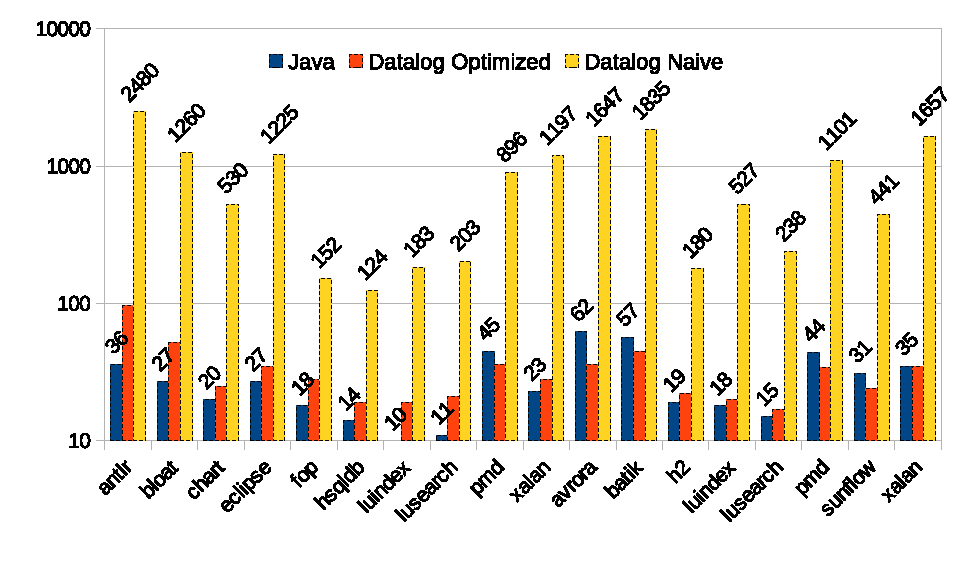
\includegraphics[clip,width=0.77\linewidth, height=0.4275\linewidth]{assets/must-data/time.eps}
\caption[Execution times for the Java and both Datalog versions]{Execution time (sec.) of the analysis. We only show the numbers for the Java and Datalog naive versions, to avoid crowding the chart.}
\label{fig:must-data:time-chart}
\end{figure*}

Note that the figure is log-scale. Across all benchmarks, the difference between the optimized implementations and the original is typically at least an order of magnitude and often close to two.  The speedup of the two optimized implementations (vs. the original) is also shown more explicitly in Figure~\ref{fig:must-data:speedup-chart}: over half the benchmarks enjoy speedups of over \nums{20x} for both the Java and the Datalog optimized implementation. The Java version of the data structure achieves a median speedup of \nums{25.7x} (min \bad{8.4x}, max \best{68.9x}), while the Datalog version has a median speedup of \nums{24.6x} (min \bad{5.4x}, max \best{47.3x}).  The analysis time typically drops from over ten minutes to under half a minute. 

\begin{figure*}[htp]
\centering
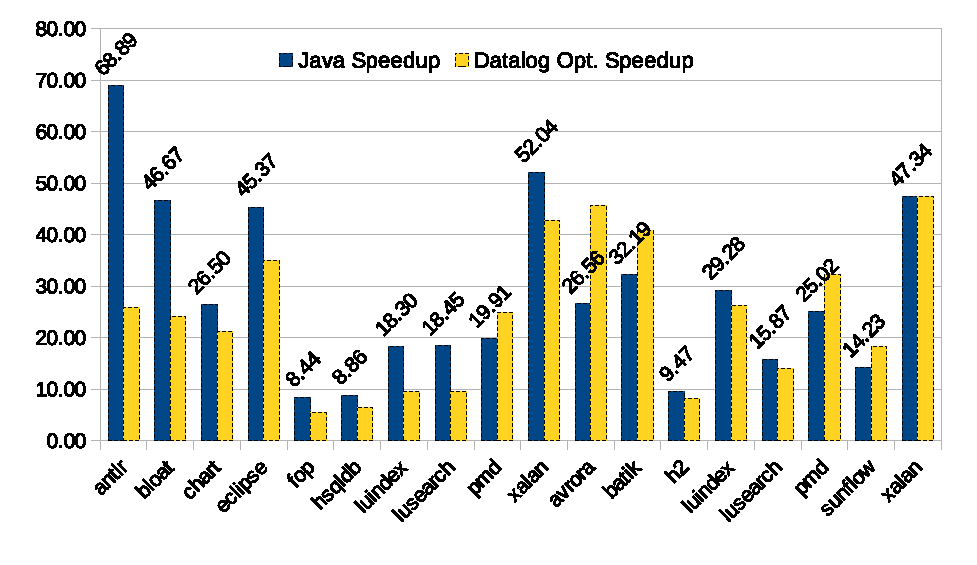
\includegraphics[clip,width=0.77\linewidth, height=0.4275\linewidth]{assets/must-data/speedup.eps}
\caption[Speedups of employing the optimized data structure]{Speedups of employing the optimized data structure.}
\label{fig:must-data:speedup-chart}
\end{figure*}

It is not hard to see why the explicit representation is not competitive. Figure~\ref{fig:must-data:pairs-chart} correlates the number of aliased access-path pairs (computed by the original analysis) and execution time. (This applies to context-qualified access paths, in the application and libraries alike, as long as the library code is reachable from application code with the given context depth.) This metric reflects the size (in tuples) of the corresponding relation in the Datalog database. It clearly suggest that maintaining access path relationships explicitly can prove quite costly.

\begin{figure*}[htp]
\centering
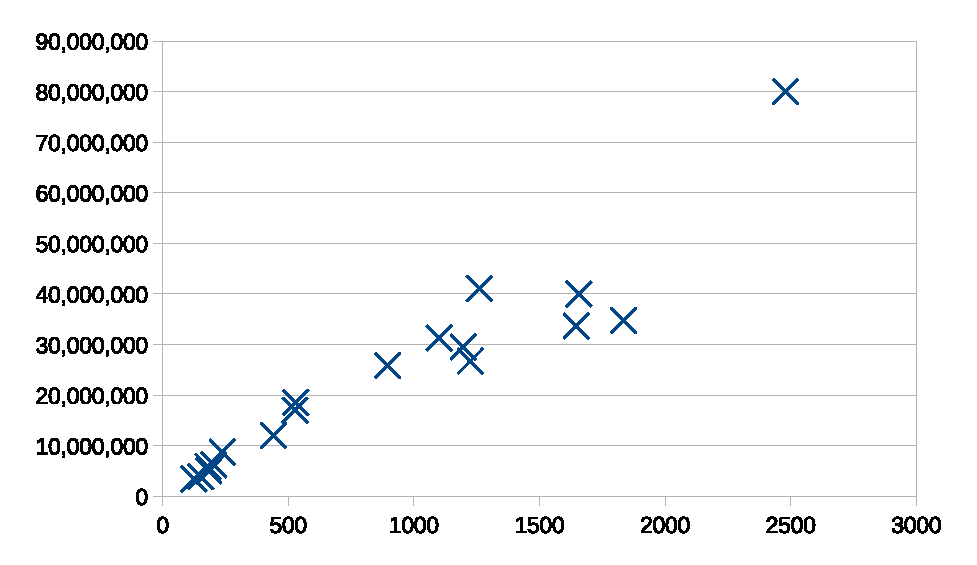
\includegraphics[clip,width=\linewidth]{assets/must-data/pairs.eps}
\caption[Number of pairs of access paths vs. analysis time]{Number of pairs of (instruction-and-context qualified) access paths that must alias vs. analysis time.}
\label{fig:must-data:pairs-chart}
\end{figure*}

Furthermore, the setup explicitly downplays the benefits of our optimized data structure: First, the ``optimized'' running time also includes import time and computing must-point-to results for checking the equivalence of analyses. The latter is quite costly, since it requires re-expanding the compactly-preserved access paths. The true computation times of the optimized analysis are about one-third of the times listed in Figure~\ref{fig:must-data:time-chart}. Second, the configuration parameters (context depth of 1 and access paths of at most length 2) are very modest, to present the explicit representation in the best possible (while still realistic) light. Changing these parameters can incur dramatic slowdowns for the explicit representation, as we examine next.


\paragraphhead{Varying access-path length.}
To further see the performance advantage of the optimized representation of must-alias information, one can vary the maximum access path length allowed for computations of the original, explicit (Datalog) implementation. Figure~\ref{fig:must-data:aplength-chart} shows how running time varies for maximum access path lengths of 2, 3 (same as in Figure~\ref{fig:must-data:time-chart}), 4 and 5. The numbers are for the xalan benchmark. The speedup readily grows to over \best{75x} for an allowed access path length of 5. The optimized Datalog implementation is shown as a baseline although it should be (and is) largely unaffected by the change of maximum access path length.

\begin{figure*}[htp]
\centering
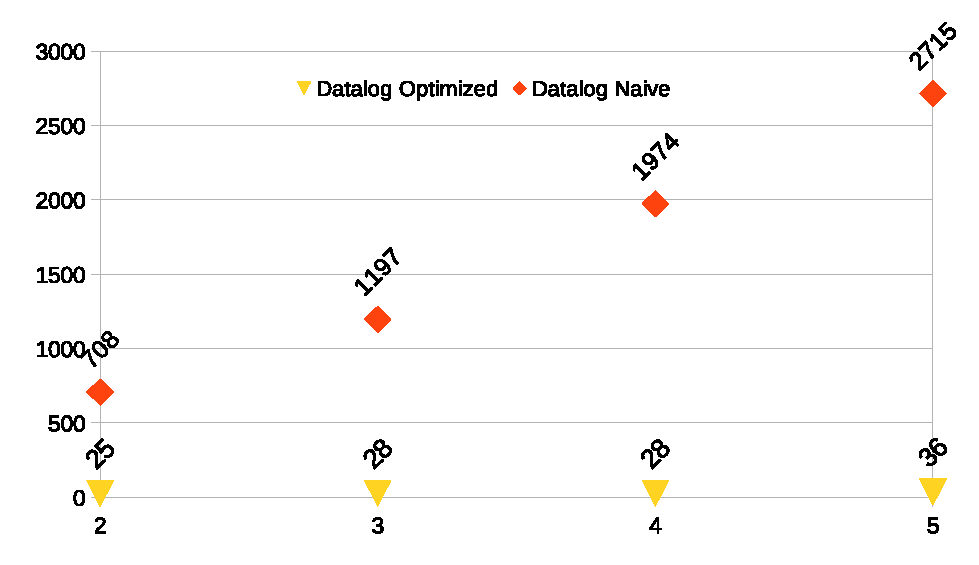
\includegraphics[clip,width=\linewidth]{assets/must-data/length.eps}
\caption[Execution times when varying max access-path length]{Execution time when varying maximum access-path length. Optimized Datalog running time given as a baseline.}
\label{fig:must-data:aplength-chart}
\end{figure*}


\paragraphhead{Varying context depth.}

\begin{figure*}[h!tp]
\centering
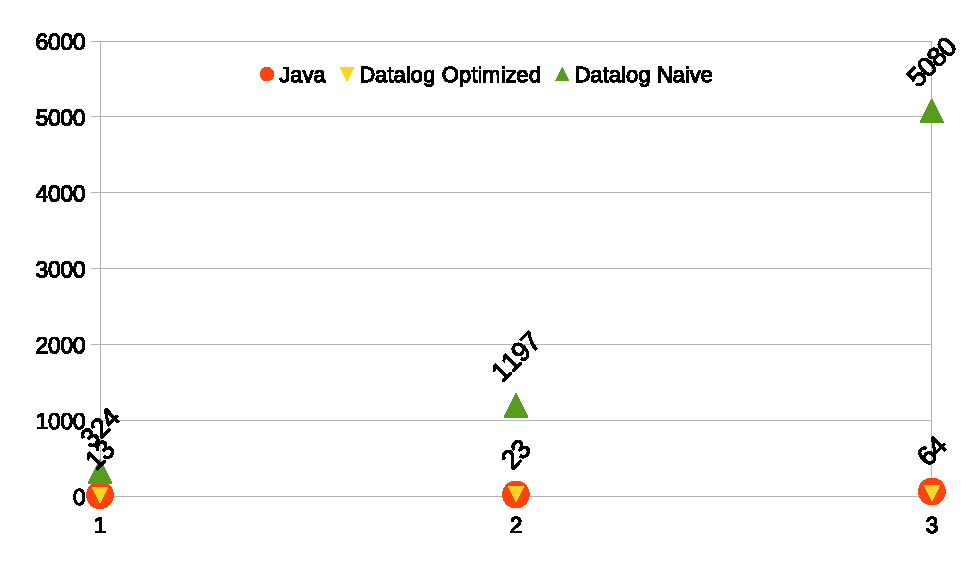
\includegraphics[clip,width=\linewidth]{assets/must-data/depth.eps}
\caption[Execution times when varying max context depth]{Execution time when varying maximum context depth.}
\label{fig:must-data:ctxdepth-chart}
\end{figure*}

Similar observations can be made by varying the context depth of the analysis. As seen in Figure~\ref{fig:must-data:ctxdepth-chart}, although the running time of the optimized implementation grows slowly, the running time of the explicit representation of alias relationships gets dramatically higher. For a context depth of 4, the explicit representation did not terminate after one-and-a-half hour.

Recall the two claimed benefits of the optimized representation: long access paths are represented implicitly, and equivalence classes are represented with linear space and time complexity, instead of quadratic. It is the latter factor that comes into play when context depth increases: alias sets grow in size, by exploiting inter-procedural inference (e.g., aliasing established at the caller and propagated through formal arguments) in addition to local instructions.


\section{Summary}

We presented a data structure for the its optimized implementation of must-alias analysis over access paths. In all, the optimized representation fulfills its promise of a much more economical representation of must-alias (equivalence) relations. The algorithmic improvements afforded by the specialized data structure yield a large performance advantage, often approaching two orders of magnitude.